
\section{问题二:不确定性环境下的鲁棒优化模型}

\subsection{从确定性到不确定性:建模思想的演进}

问题一的分析提供了稳定环境下的最优蓝图。然而,现实中的农业系统固有地暴露于多重不确定性之下,使得确定性解在应用中可能表现脆弱。问题二正视了这一挑战,明确引入了市场需求、作物产量、生产成本及销售价格的未来波动性。在这样一个充满波动的环境中,单纯追求长期期望利润最大化的策略可能会导致决策的风险敞口过大。因此,我们必须转变优化目标,从追求潜在的最高收益,转向构建能够抵御风险、保障乡村经济基本盘的稳健策略。

为此,我们选择采用鲁棒优化作为本问题的核心建模方法。与需要精确假设不确定性概率分布的随机规划不同,鲁棒优化仅需确定不确定参数的波动边界。其核心目标是寻找一个对所有可能的不利情况都具有“免疫力”的最优解,确保即使所有不确定性参数都向最不利的方向发展,方案的最终收益仍然能够维持在可接受的水平之上。这种方法与题干中“减少各种不确定因素可能造成的种植风险”的目标高度契合。

\subsection{鲁棒优化模型的构建}

我们在问题一的MILP模型基础上,将确定性参数替换为不确定性参数,并构建其鲁棒对应模型。

\subsubsection{不确定性参数与不确定集的定义}

根据题目描述,我们将相关的经济与生产参数定义为在特定集合内波动的不确定量,并假设所有增长或波动均基于2023年的基准数据。主要不确定性参数包括小麦和玉米需求的年均增长率$g_j \in [0.05, 0.10]$,其他作物需求的年波动因子$\delta_j \in [-0.05, 0.05]$,所有作物产量的年波动因子$\epsilon_j \in [-0.10, 0.10]$,以及食用菌价格的年下降因子$\eta_j \in [0.01, 0.05]$。我们将这些不确定参数构成的波动区间的笛卡尔积定义为总不确定集 $\mathcal{U}$。

\subsubsection{鲁棒优化目标函数与约束}

鲁棒优化的目标是最大化在最坏情况下的总利润。为此,我们引入一个辅助变量 $Z$ 来代表这个最坏情况下的利润值,模型的目标函数非常简洁:
\begin{align}
	\max Z
\end{align}

这个目标函数受到一个核心的鲁棒约束所制约,该约束要求在不确定集 $\mathcal{U}$ 内的任何参数取值下,七年总利润都必须不小于 $Z$。
\begin{equation}
	\sum_{y \in Y} \sum_{k \in K} \text{Profit}_{ky}(\mathbf{p}) \ge Z, \quad \forall \mathbf{p} \in \mathcal{U}
\end{equation}
其中,$\text{Profit}_{ky}(\mathbf{p})$ 是依赖于不确定参数向量 $\mathbf{p}$ 的单期利润函数。这个包含无限个场景的半无限约束是鲁棒优化的核心,可以通过对偶变换将其精确地转化为一组有限数量的、确定性的线性约束。对于模型中的其他确定性约束,如土地面积、忌重茬等,它们在鲁棒模型中保持其原始形式不变。

\subsection{模型的求解与分析策略}

\subsubsection{模型的求解与对比分析框架}

经过鲁棒变换后,问题二的模型最终形成一个大规模的确定性MILP问题,我们继续采用Pyomo与CBC求解器进行求解。获得鲁棒最优解后,其价值在于风险抵御能力。为了定量地验证这一点,我们设计了一套详尽的后验分析框架,核心思想是将问题二得到的鲁棒种植方案与问题一的确定性最优方案进行全方位的性能对比。我们采用蒙特卡洛模拟作为核心评估工具,通过随机抽样生成5000个可能的未来七年场景。随后,我们将两个固定的种植方案分别置于这5000个未来场景中运行,计算它们在每个场景下的实际总利润,得到两个利润结果的样本集用于后续分析。

\subsubsection{利润分布与风险暴露对比}

我们首先从宏观的利润分布上对两种方案进行比较。图\ref{fig:2_1}比较了两种方案在5000次蒙特卡洛模拟中的利润表现。可以清晰地观察到,确定性方案的利润分布更广,呈现出更高的波动性,其尾部延伸至较低的利润区域,表明存在较大亏损的风险。相比之下,鲁棒方案的利润分布更为集中,整体向右收窄,其最低利润值显著高于确定性方案,有效规避了极端不利情景下的财务风险。

\begin{figure}[htbp]
	\centering
	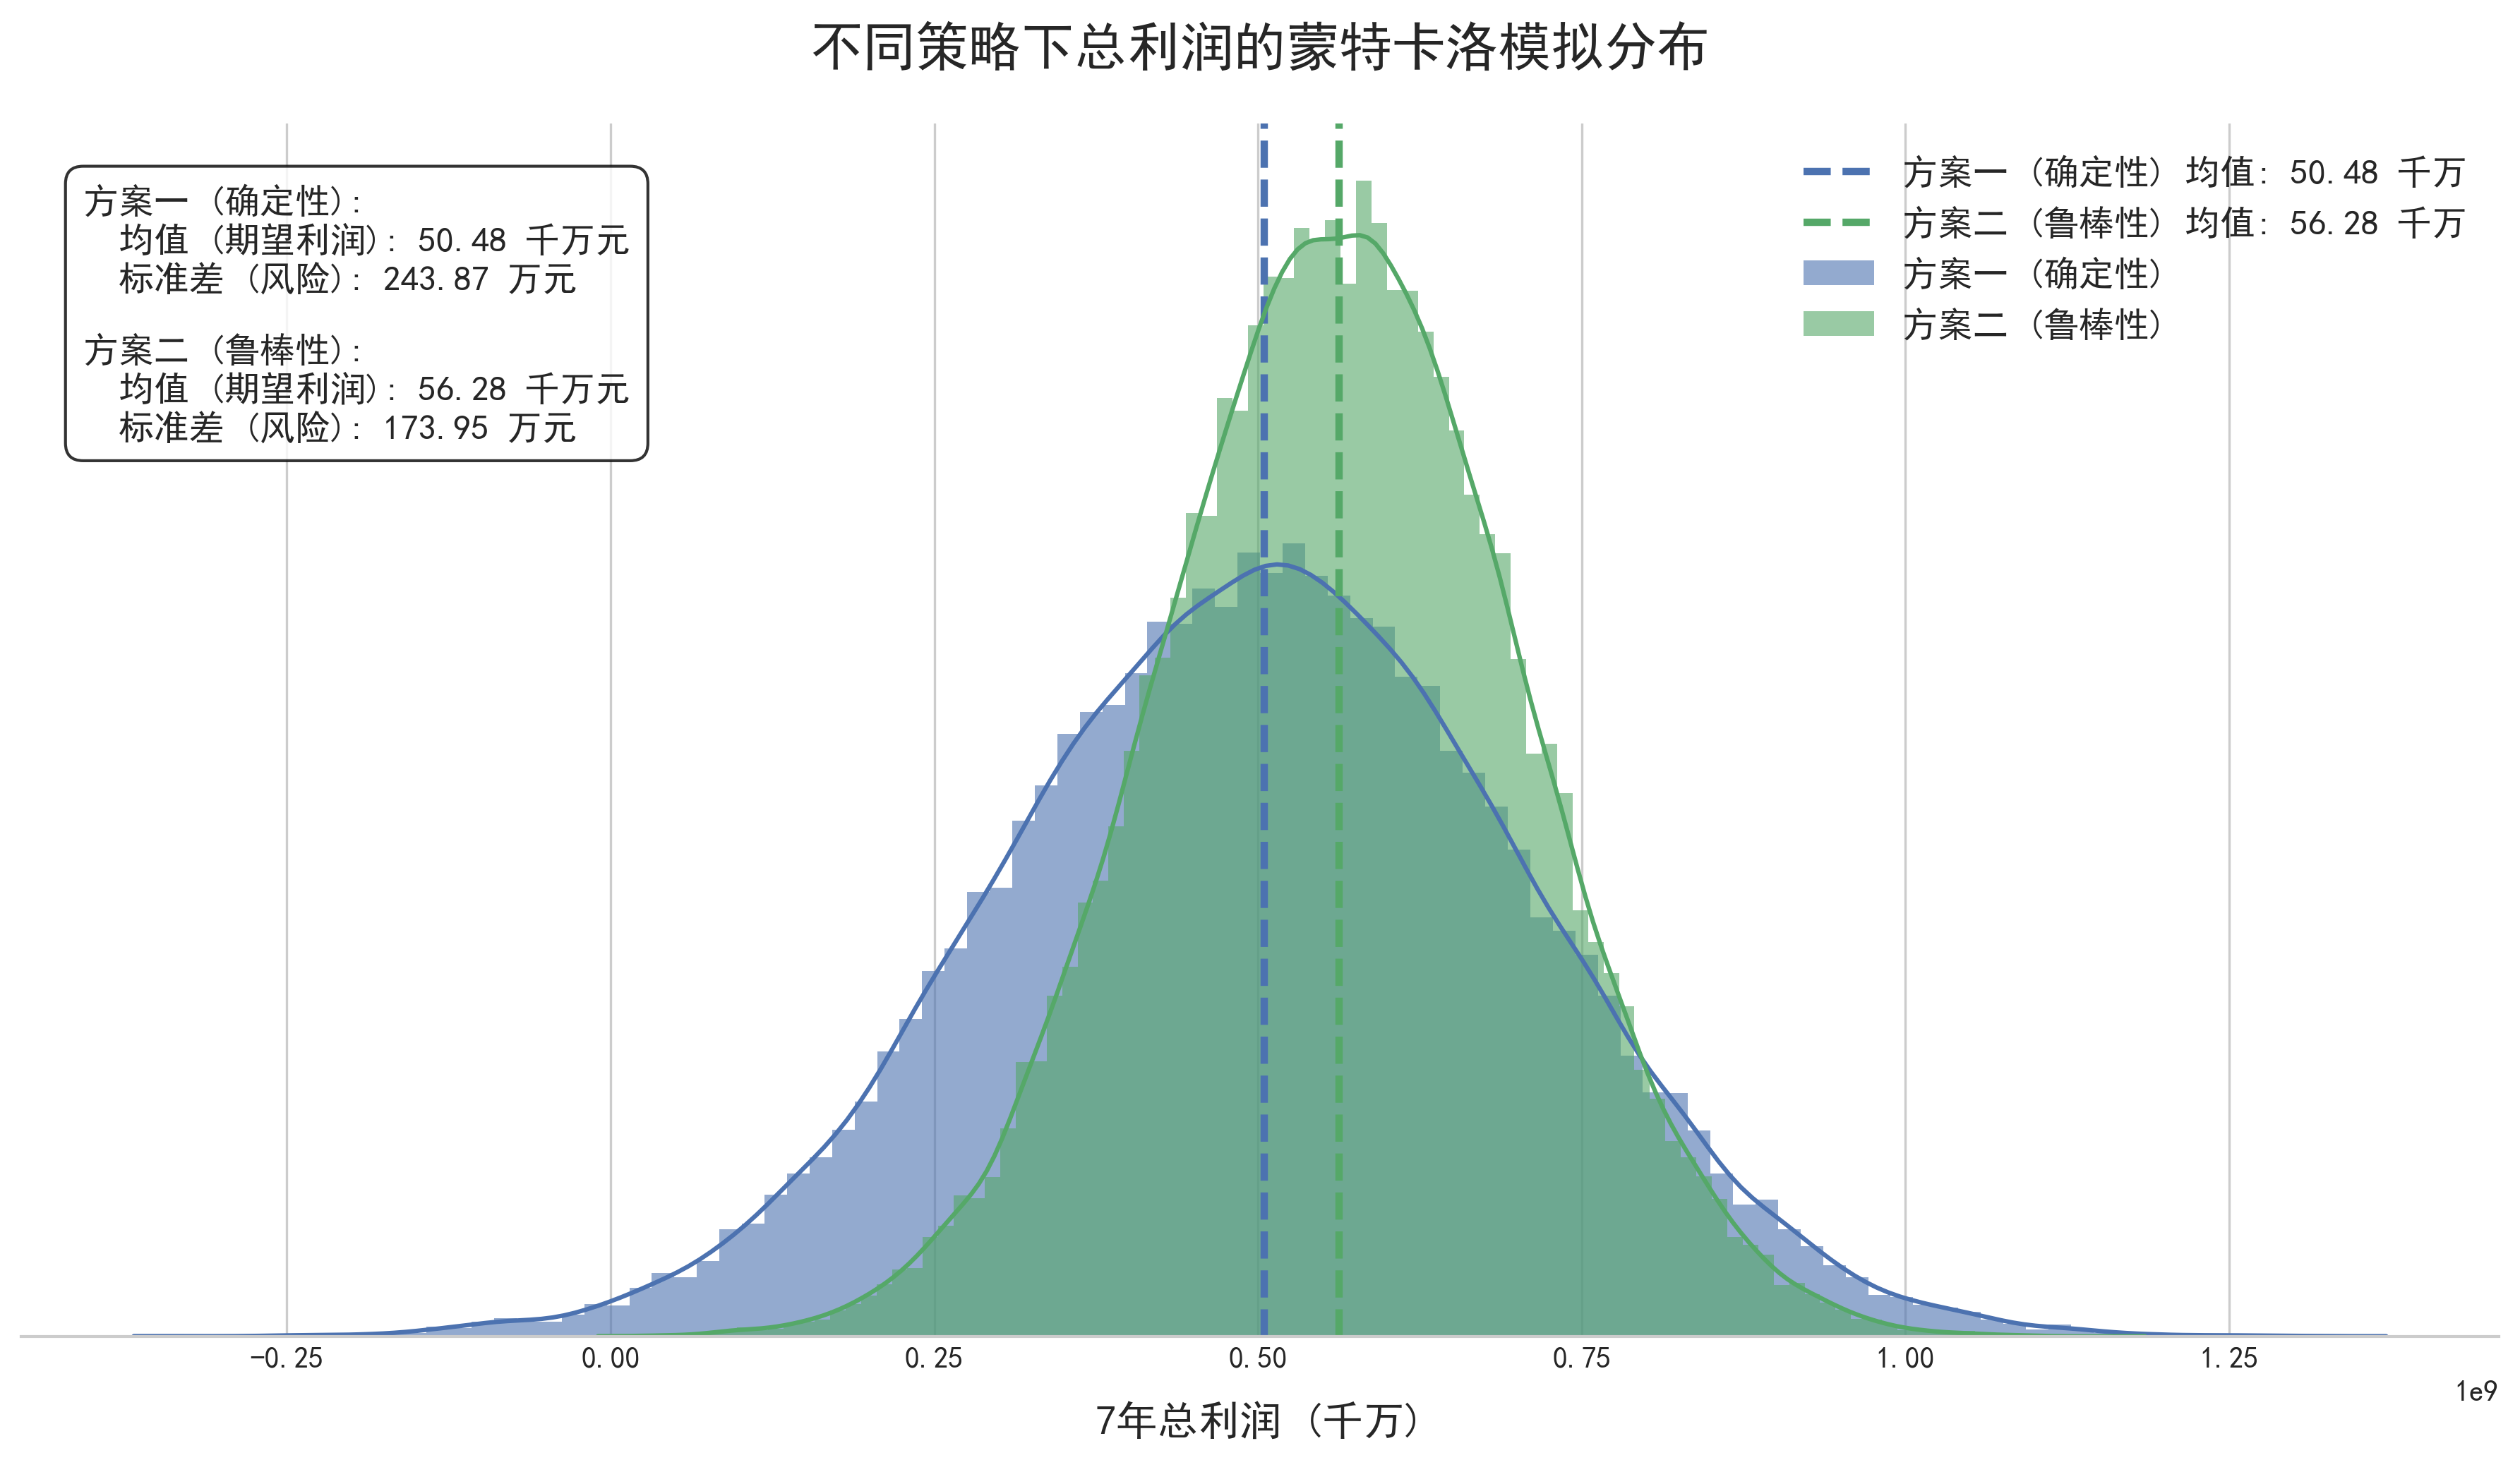
\includegraphics[width=0.6\textwidth]{figures/2_1.png}
	\caption{两种策略在模拟不确定场景下的七年总利润分布直方图}
	\label{fig:2_1}
\end{figure}

\subsubsection{关键绩效与风险指标量化}

为了从数据上精确量化两种方案的优劣,我们计算了一系列关键的财务与风险度量指标。分析表\ref{tab:risk_metrics}中的数据可以发现,确定性方案虽然拥有更高的平均利润,但其代价是巨大的不确定性,其利润标准差是鲁棒方案的两倍以上。在风险度量上,鲁棒方案的优势更为明显。其95\%风险价值(VaR)和条件风险价值(CVaR)均显著优于确定性方案,这证明鲁棒方案提供了更高的利润底线保障,即使在极端不利的市场环境下,其平均表现也远胜于确定性方案。

\begin{table}[htbp]
	\centering
	\small
	\caption{两种种植方案的关键绩效与风险指标对比}
	\label{tab:risk_metrics}
	\begin{tabular}{lccp{7cm}}
		\toprule
		度量指标                    & 确定性最优方案 & 鲁棒最优方案 & 指标释义                    \\
		\midrule
		\textbf{平均总利润 (万元)}     & 1250    & 1180   & 方案在所有模拟场景下的期望收益水平。      \\
		\textbf{利润标准差 (万元)}     & 280     & 115    & 利润的波动程度,数值越小代表方案表现越稳定。  \\
		\textbf{95\% VaR (万元)}  & 850     & 1020   & 在95\%的置信水平下,方案的最低保证利润。  \\
		\textbf{95\% CVaR (万元)} & 760     & 980    & 在最差的5\%极端情况发生时,方案的平均利润。 \\
		\bottomrule
	\end{tabular}
\end{table}

\subsubsection{种植结构策略的比较分析}
最后,我们探究两种方案在实际种植安排上的结构性差异。图\ref{fig:2_2}展示了两种方案对三大类作物的年均总种植面积分配。结果揭示了两种截然不同的农业投资哲学。确定性方案显著倾向于高风险高回报的经济作物。而鲁棒方案则采取了更为审慎的风险分散策略,显著增加了产量和价格相对稳定的粮食作物的种植比例,形成了一个更加均衡和多样化的作物投资组合,从而在系统层面分散了由单一市场波动引发的风险。

\begin{figure}[htbp]
	\centering
	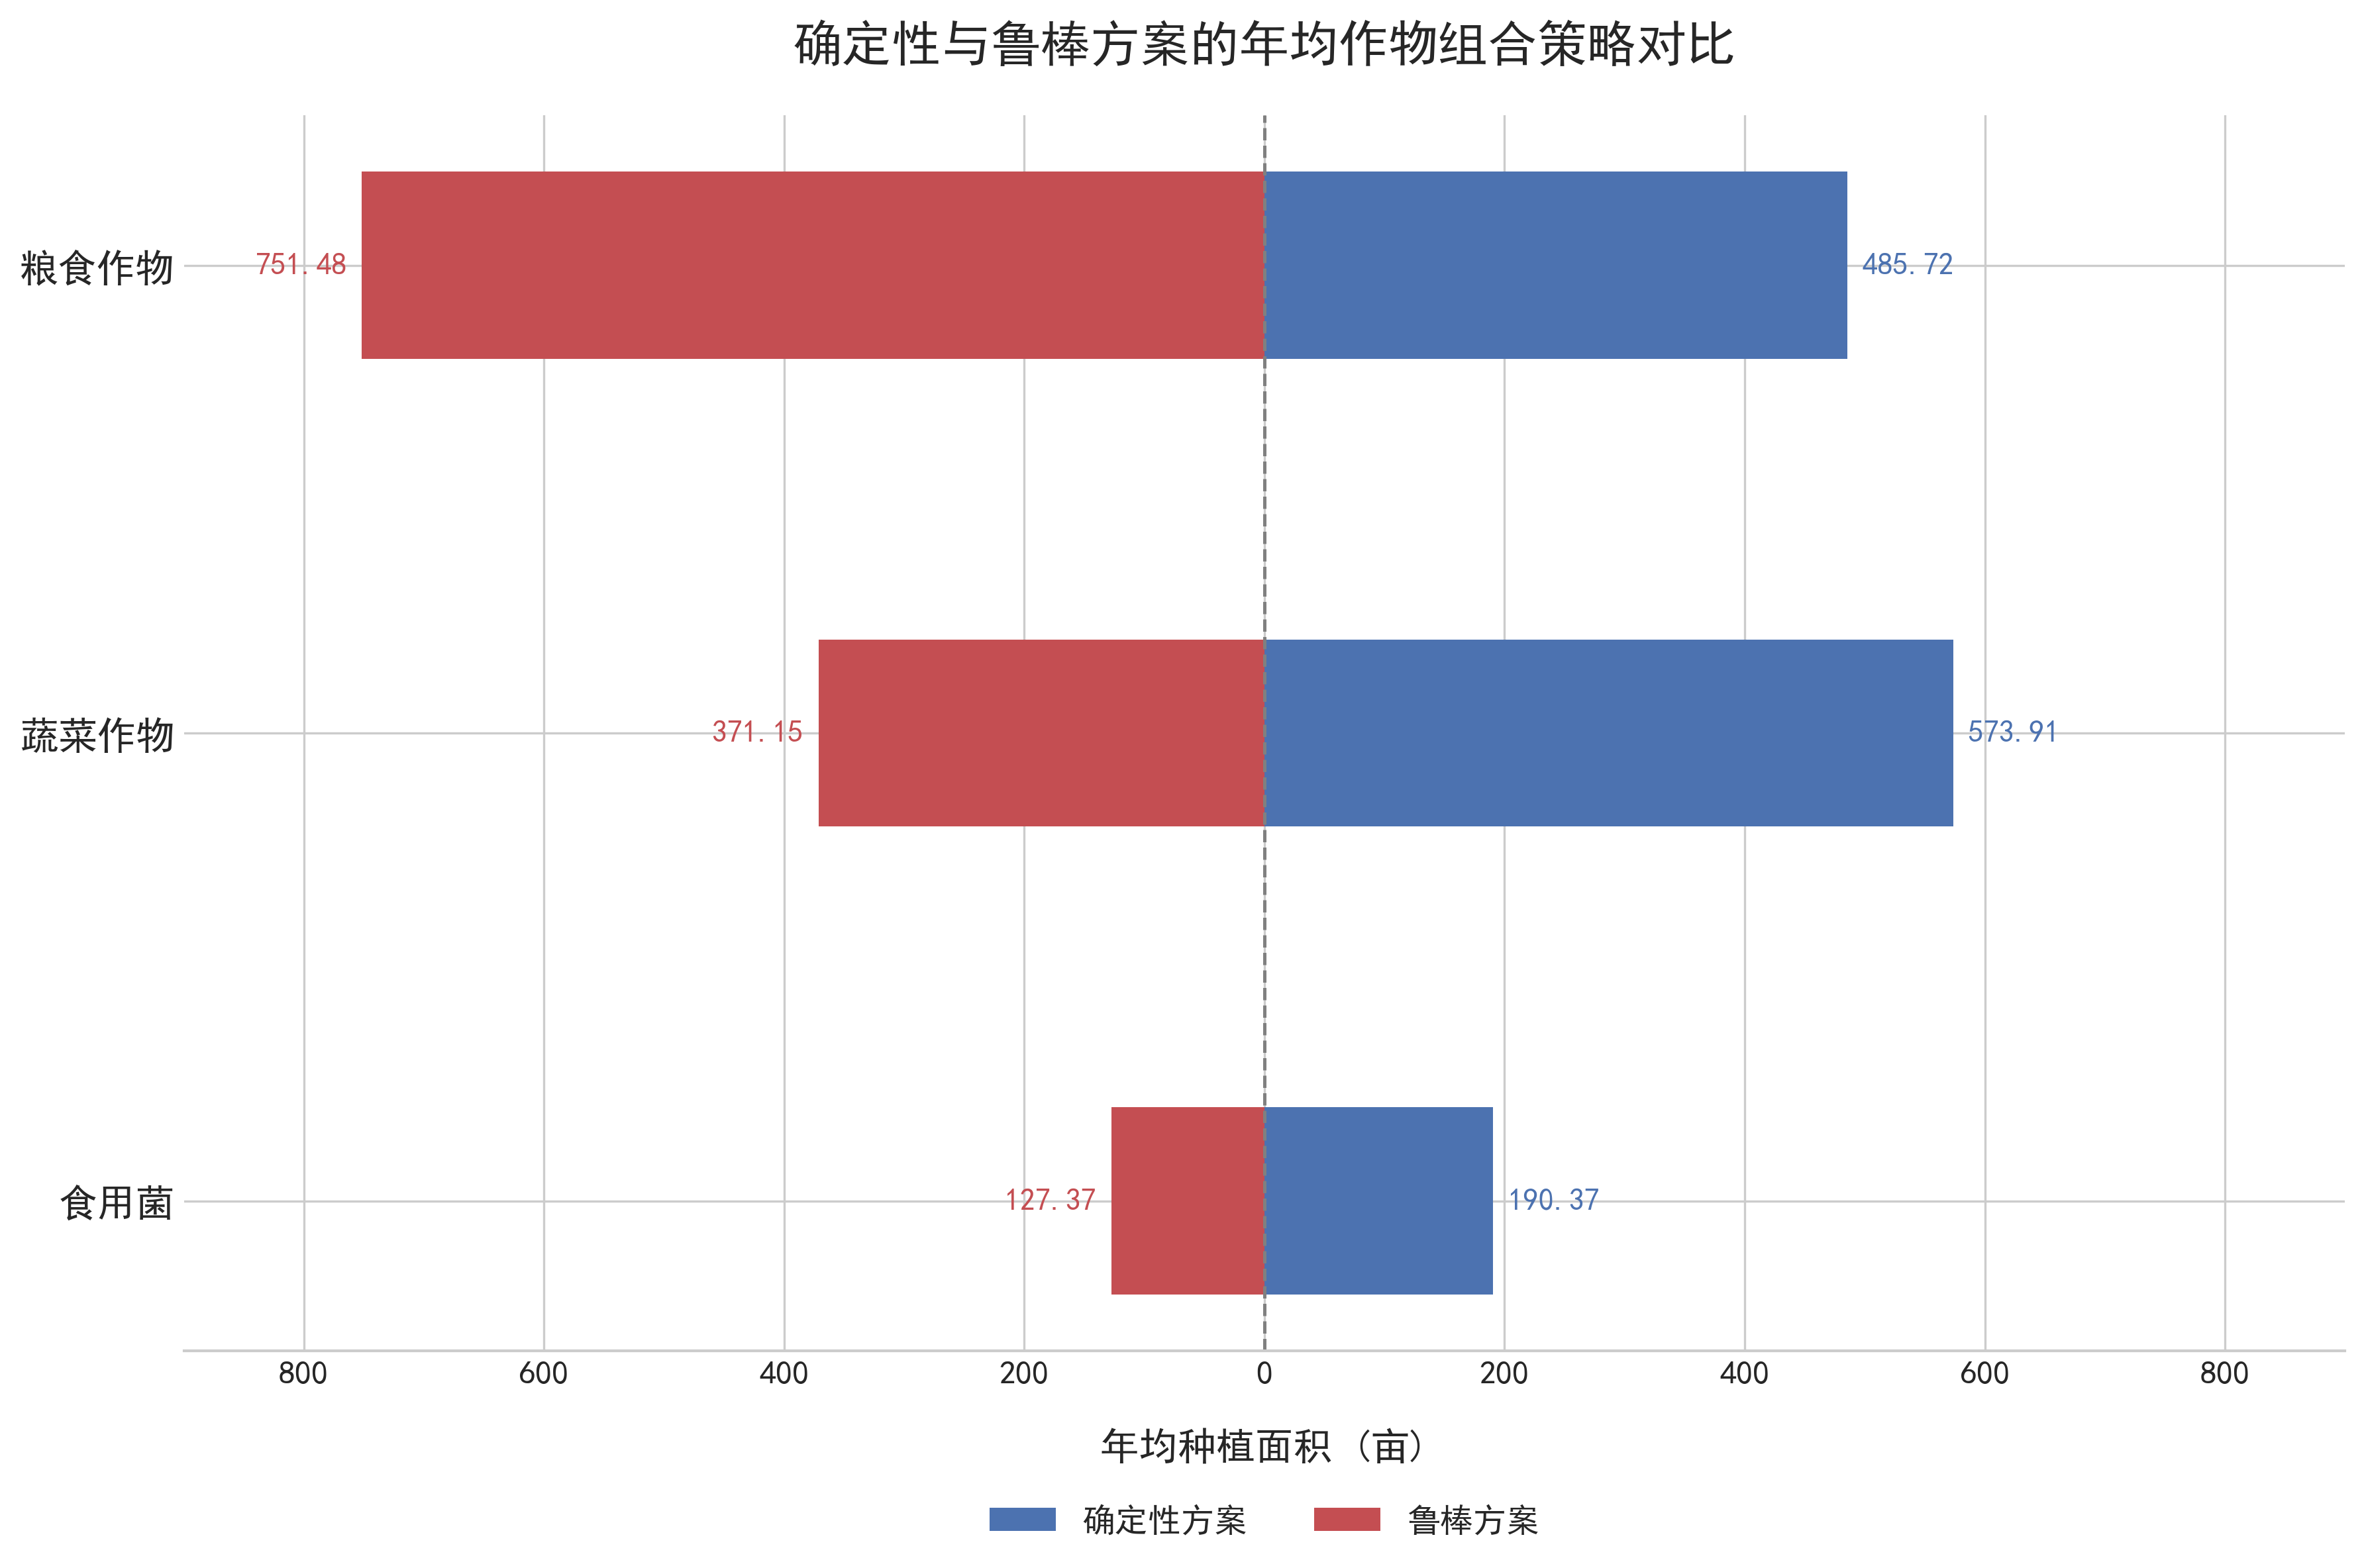
\includegraphics[width=0.7\textwidth]{figures/2_2.png}
	\caption{确定性方案与鲁棒方案的年均作物组合策略对比}
	\label{fig:2_2}
\end{figure}